In diesem Kapitel werden die durchgeführten Simulationen dokumentiert.

Zur Simulation wird das Tool \dq Xpedition AMS\dq\ von Siemens verwendet. Wie der Name sagt, unterstützt dieses Tool
\acrfull{ams} Analyse. \cite{siemens2025xpeditionams}

\subsection{Laser Treiber}

In Abbildung~\ref{fig:simulation_laser_driver_schematic} ist das Schema für die Simulation des Laser-Treibers
dargestellt. Dies entspricht der Schaltung aus Kapitel~\ref{sec:schematic_laser_driver}.

\begin{figure}[H]
    \centering
    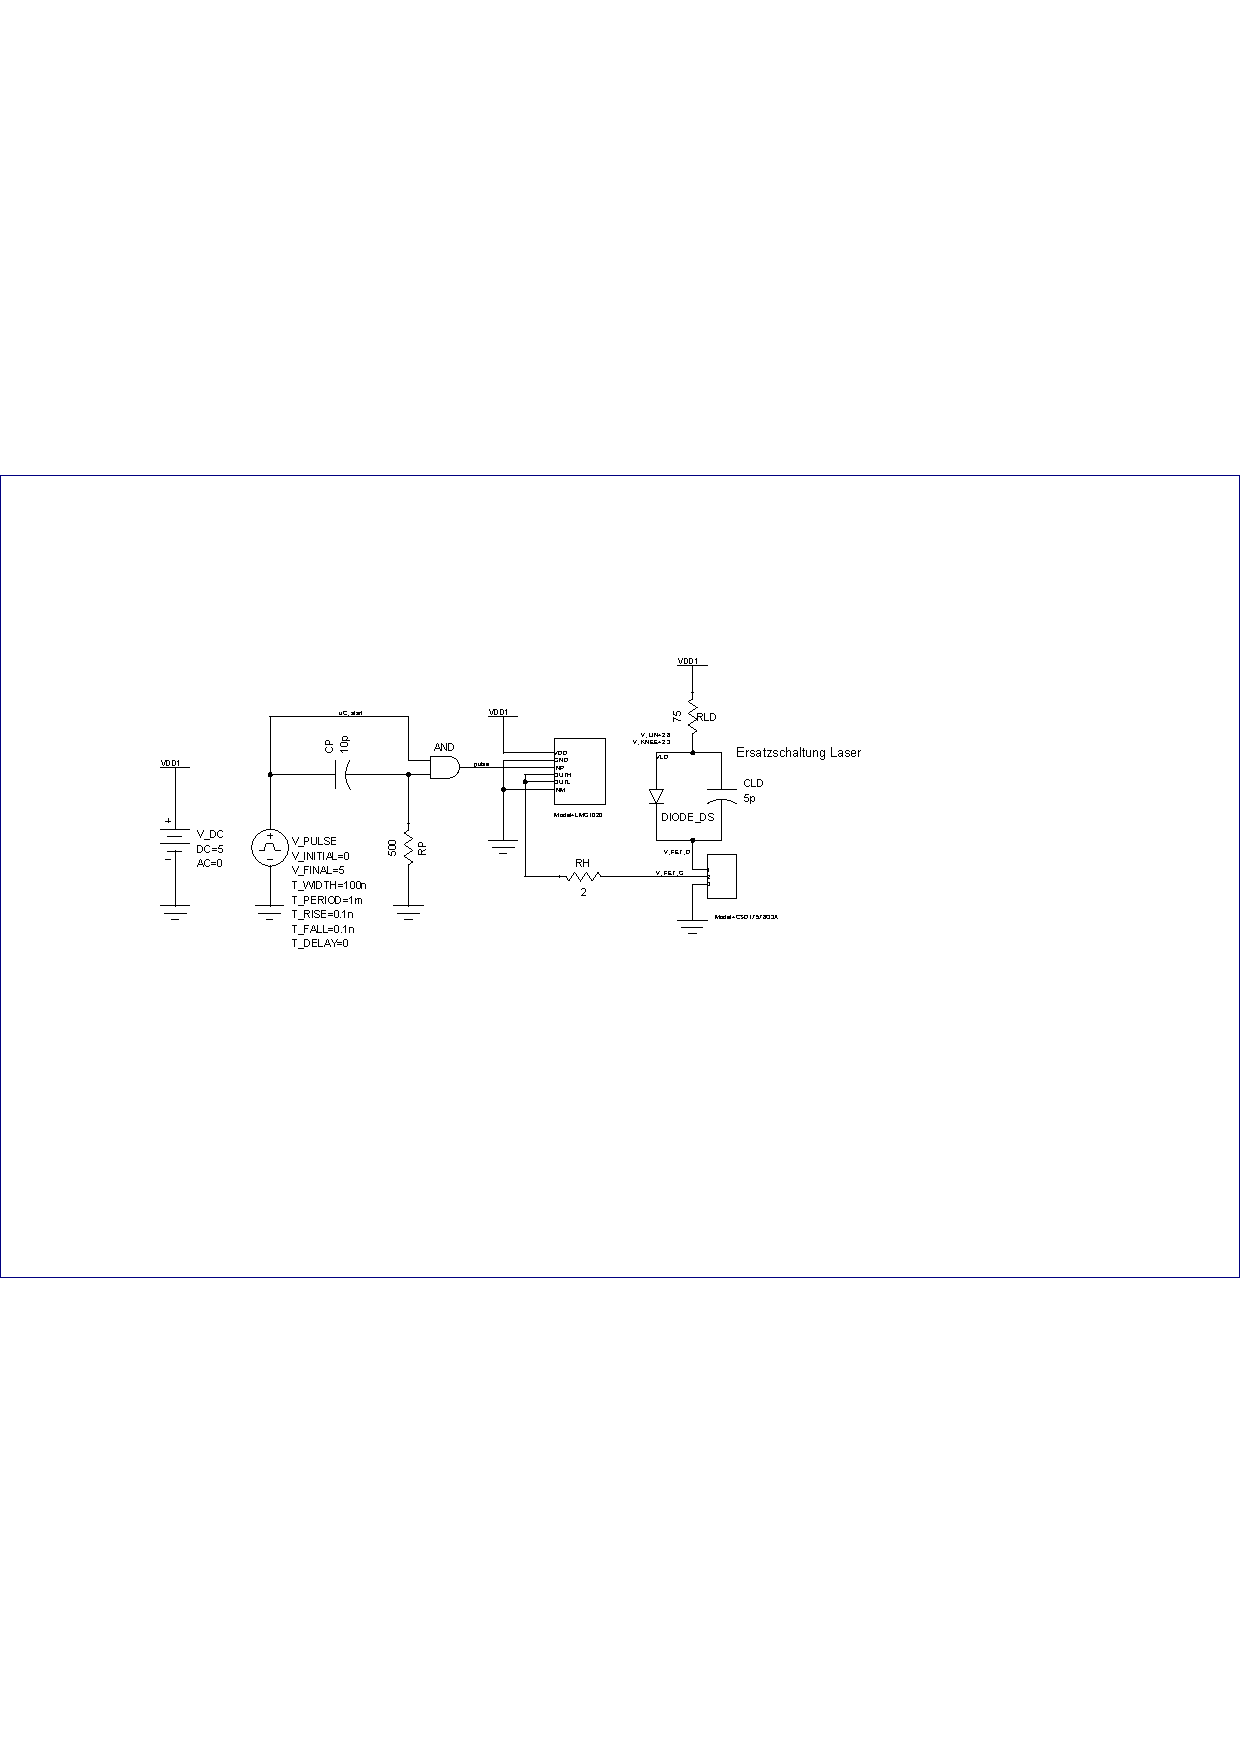
\includegraphics[trim=70 380 180 310, clip, width=0.9\textwidth]{attachments/simulation_laser_driver_schematic.pdf}
    \caption{Simulation Laser-Treiber - Schema}\label{fig:simulation_laser_driver_schematic}
\end{figure}

Das SPICE-Modell des Gate-Treibers LMG1025-Q1 ist dasselbe wie für LMG1020 und wurde von der Website von TI
heruntergeladen \cite{ti2024lmg1025q1}.

Das SPICE-Modell des NexFET CSD17578Q3A wurde ebenfalls von der Website von TI heruntergeladen
\cite{ti2024csd17578q3a}.

Für die Laser-Diode RLD65NZX1 konnte kein SPICE-Modell gefunden werden, es wurde deshalb eine Ersatzschaltung aus Diode
und paralleler, parasitärer Kapazität eingefügt.

Das Resultat der Simulation ist in Abbildung~\ref{fig:simulation_laser_driver_plot} dargestellt.

\begin{figure}[H]
    \centering
    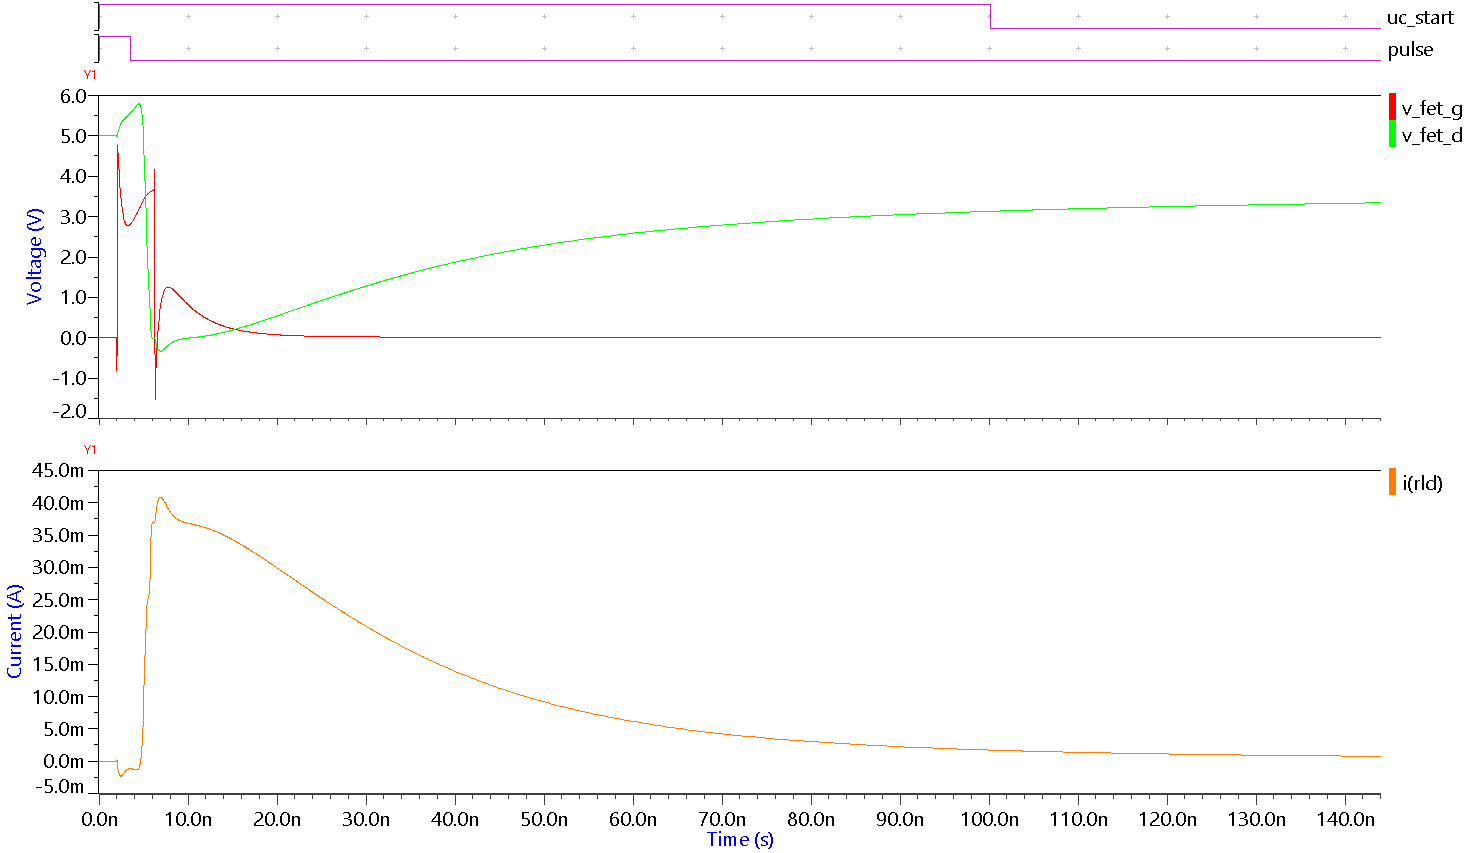
\includegraphics[width=\textwidth]{graphics/simulation_laser_driver_plot.png}
    \caption{Simulation Laser-Treiber - Plot}\label{fig:simulation_laser_driver_plot}
\end{figure}

Es ist zu erkennen, dass der Laser sehr schnell einschalten kann (2 \dots 3~ns). Das Ausschalten dauert etwas länger
(ca. 100~ns). Da die \acrshort{tof} bis zur ersten Flanke gemessen wird, ist eine längere Ausschaltzeit für diese
Anwendung kein Problem.

\subsection{Transimpedanzverstärker}

In Abbildung~\ref{fig:simulation_tia_schematic} ist das Schema für die Simulation des Transimpedanzverstärkers
dargestellt. Dies entspricht der Schaltung aus Kapitel~\ref{sec:schematic_photo_receiver}, ohne den Komparator.

\begin{figure}[H]
    \centering
    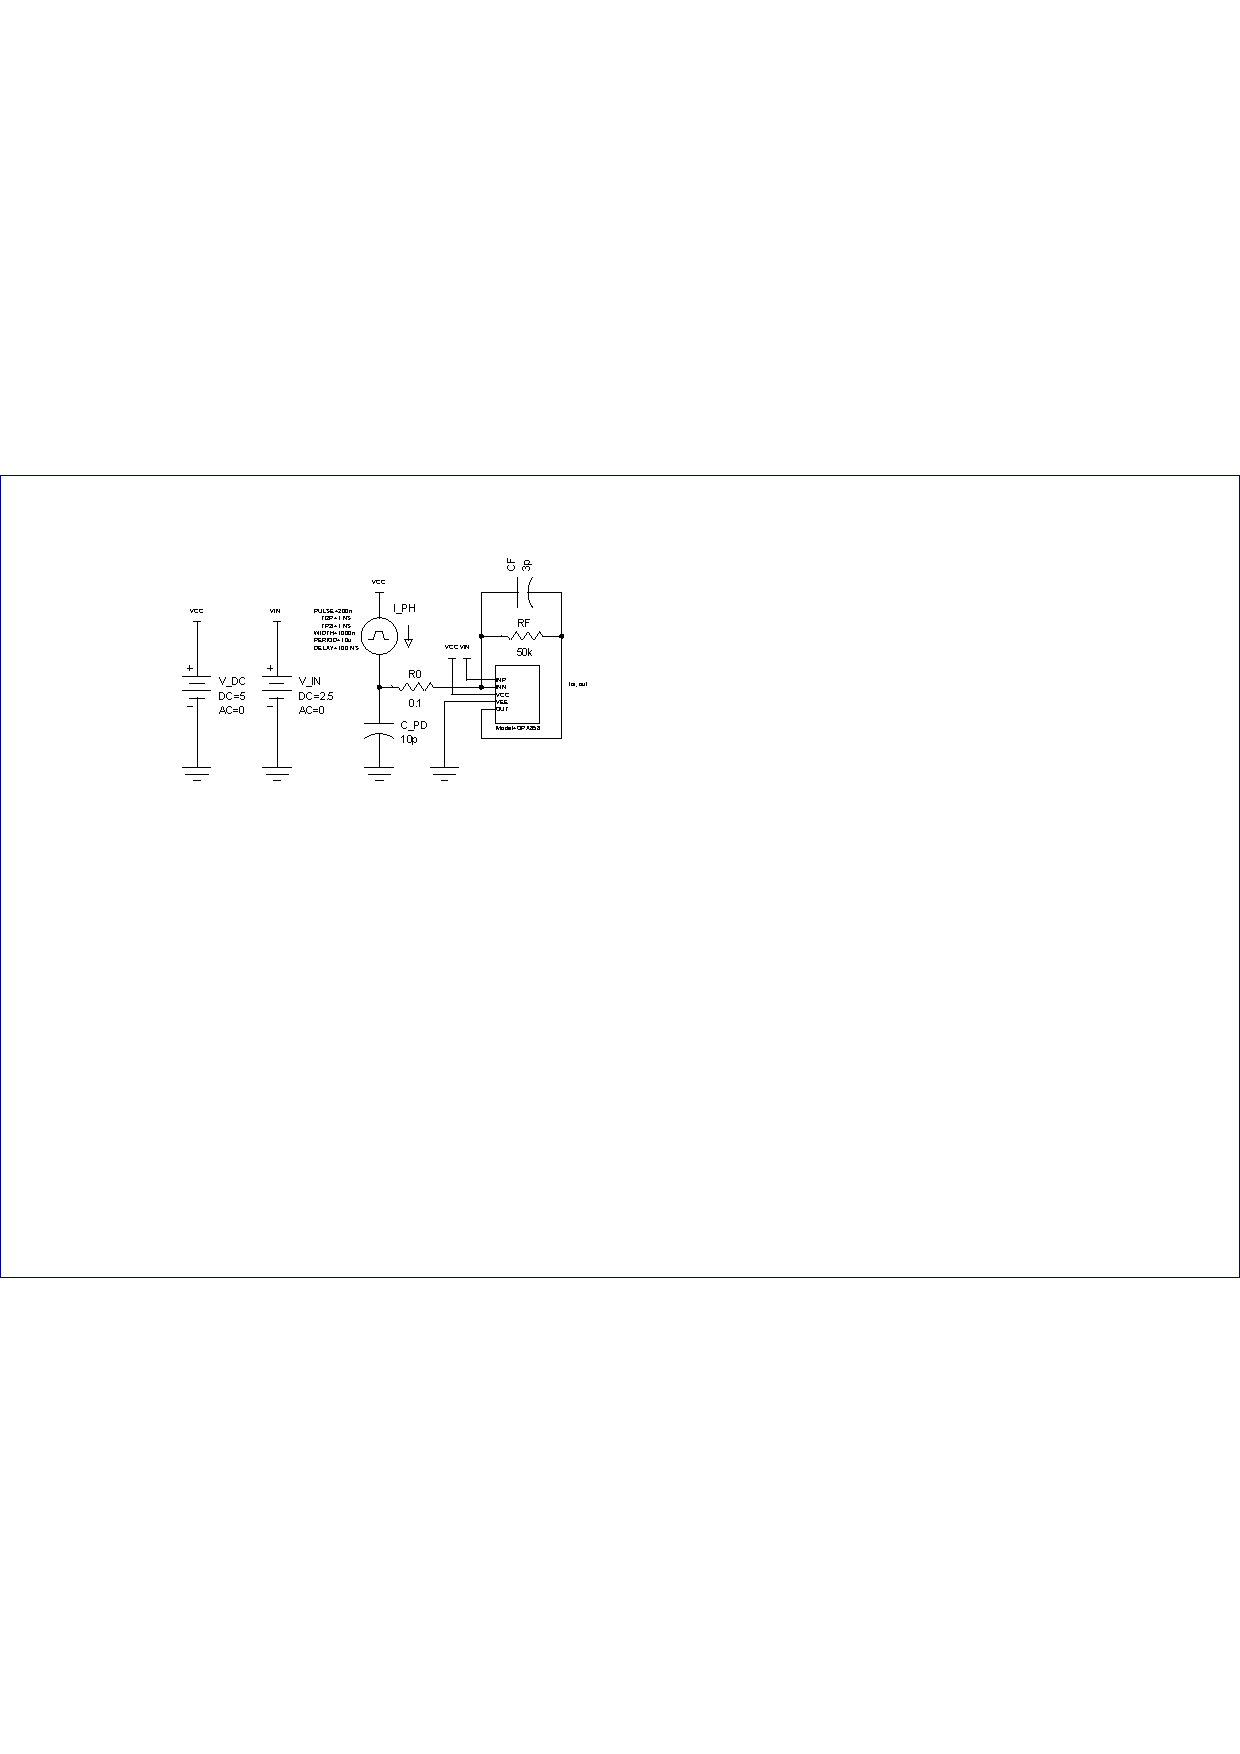
\includegraphics[trim=80 465 310 265, clip, width=0.7\textwidth]{attachments/simulation_tia_schematic.pdf}
    \caption{Simulation \acrshort{tia} - Schema}\label{fig:simulation_tia_schematic}
\end{figure}

Das SPICE-Modell des Operationsverstärkers OPA858 wurde von der Website von TI heruntergeladen \cite{ti2024opa858}.

Für die Photo-Diode NJL6401R konnte kein SPICE-Modell gefunden werden, es wurde deshalb eine Ersatzschaltung aus
Strompuls-Quelle und paralleler, parasitärer Kapazität eingefügt.

Das Resultat der Simulation ist in Abbildung~\ref{fig:simulation_tia_plot} dargestellt.

\begin{figure}[H]
    \centering
    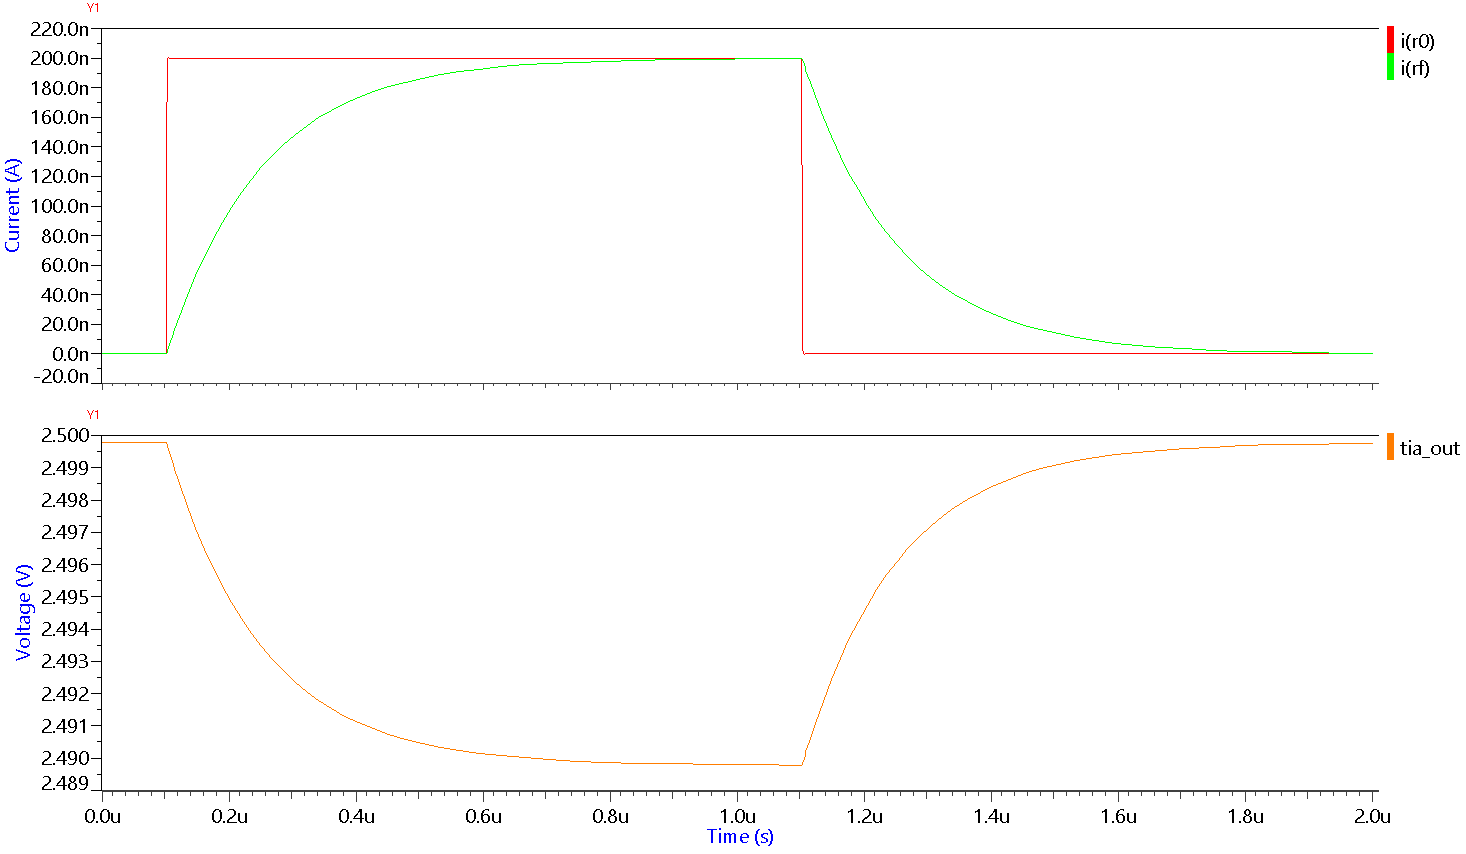
\includegraphics[width=\textwidth]{graphics/simulation_tia_plot.png}
    \caption{Simulation \acrshort{tia} - Plot}\label{fig:simulation_tia_plot}
\end{figure}

Es ist zu erkennen, dass die Zeitkonstante des Stroms durch den Feedback-Widerstand \lstinline|RF| gemäss
Formel~\ref{eq:tia_tau} bestimmt werden kann.

\begin{equation}\label{eq:tia_tau}
    \tau = R_F \cdot C_F = 50~k\Omega \cdot 3~pF = 150~ns
\end{equation}
\myequations{\acrshort{tia} Zeitkonstante}

Beliebig klein kann der Feedback-Kondensator \lstinline|CF| jedoch nicht gewählt werden, da die Schaltung sonst schwingt.

In Abbildung~\ref{fig:simulation_tia_plot_wo_cf} ist das Simulations-Resultat ohne den Feedback-Kondensator
\lstinline|CF| dargestellt.

\begin{figure}[H]
    \centering
    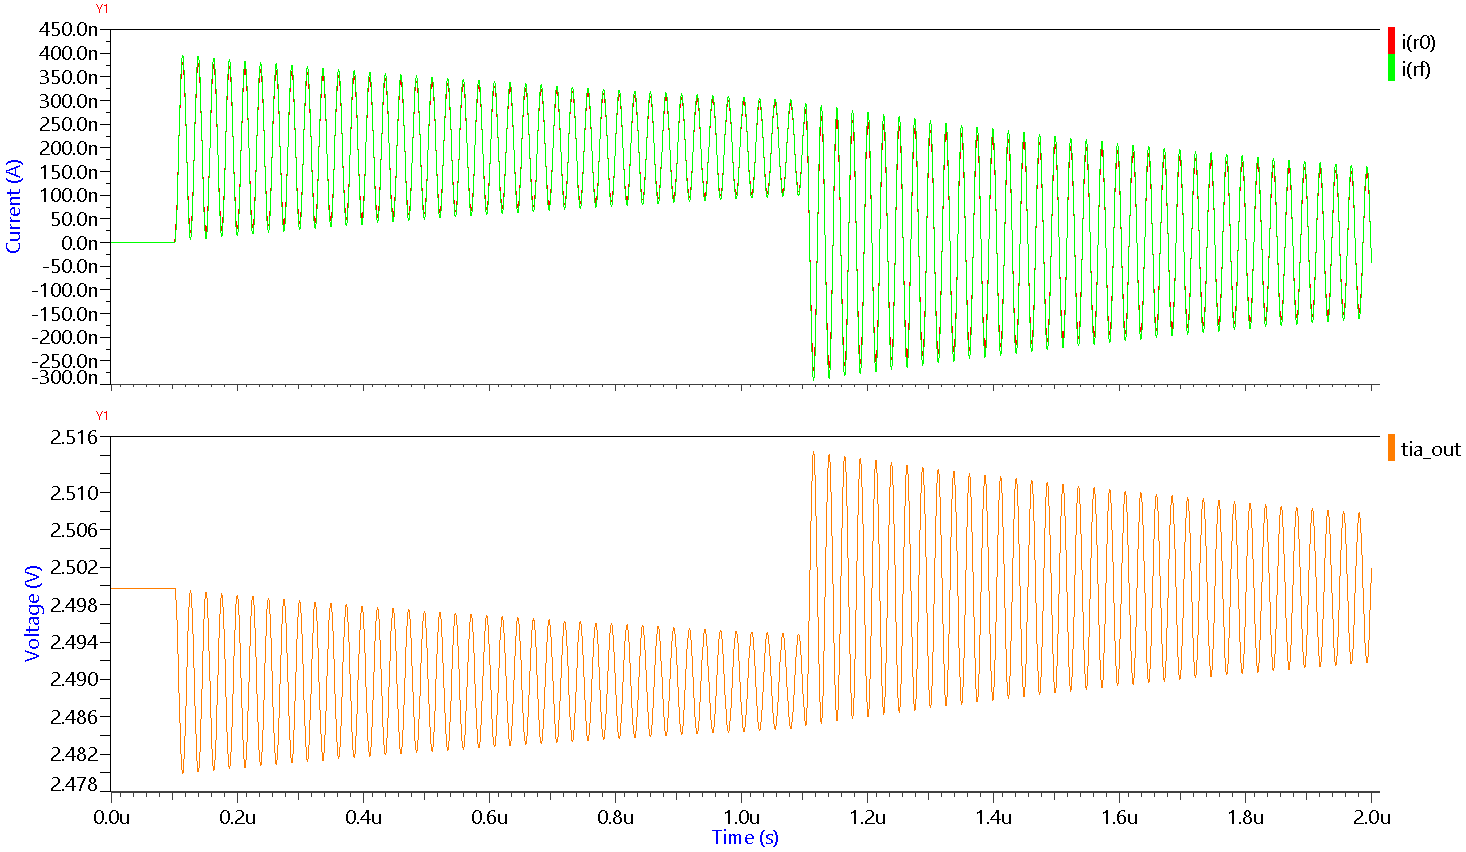
\includegraphics[width=\textwidth]{graphics/simulation_tia_plot_wo_cf.png}
    \caption{Simulation \acrshort{tia} - Plot ohne \lstinline|CF|}\label{fig:simulation_tia_plot_wo_cf}
\end{figure}

Die genaue Dimensionierung von \lstinline|CF| wird durch Tests mit dem \acrshort{pcb} bestimmt werden. Eventuell, je
nach parasitären Kapazitäten auf dem \acrshort{pcb}, wird \lstinline|CF| auch gar nicht bestückt werden müssen.
